\documentclass[12pt, a4paper]{article}

% Packages
\usepackage[margin=1in]{geometry}
\usepackage{graphicx}
\usepackage{hyperref}
\usepackage[utf8]{inputenc}
\usepackage[english,serbian]{babel}
\usepackage{graphicx}
\usepackage[labelformat=empty]{caption}

% Title and author information
\title{Optimizacija problema sečenja}
\author{\small Veljko Prodan \and \small Maja Milenković}
\date{}

\begin{document}

\maketitle


\section{Uvod}
Ovaj rad se bavi optimizacijom problema sečenja uz pomoć simuliranog kaljenja i genetskog algoritma. Za testiranje algoritama korišćen je 21 test primer, svaki različite dužine. Test primeri do određene dužine su testirani CPLEX rešavačem radi poređenja sa genetskim algoritmom i simuliranim kaljenjem, kao i kombinacijom ova dva algoritma.

\section{Problem sečenja}
Problem sečenja (Cutting stock problem - CSP) je NP težak problem u kojem je cilj naći najbolji način da se materijal određenih dimenzija iseče na manje komade zadatih dimenzija, tako da se minimizuje otpad i poveća iskorišćenost materijala. Ovaj problem se često javlja u industriji papira, čelika, drveta, tekstila i sl. Rešavanje ovog problema je složeno zbog velikog broja mogućih kombinacija isecanja narudžbina.

U ovom radu, za dužinu jednog komada materijala je korišćena fiksna vrednost od 100 cm, a rešenje problema je predstavljeno kombinacijom zadatih celih brojeva između 1 i 100. Vrednost jednog rešenja se računa tako što se lista otpadaka jedne narudžbine sortira u opadajućem poretku pa se zatim dužina svakog otpatka pomnoži sa svojom pozicijom u sortiranoj listi. Zbir dobijenih vrednosti predstavlja vrednost datog rešenja. \\

\begin{minipage}{\linewidth}
    \centering
    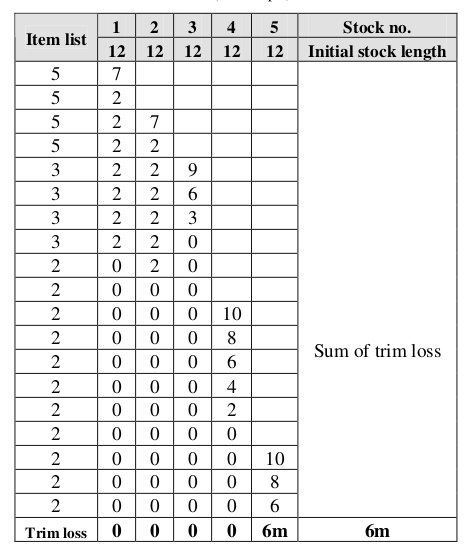
\includegraphics[width=0.5\linewidth]{img/predstavak_resenja.png}
\end{minipage}

%\clearpage

\begin{figure}[h]
    \centering
    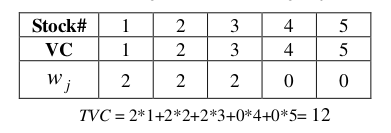
\includegraphics[width=0.45\linewidth]{img/vrednost_resenja_1.png}\hfill
    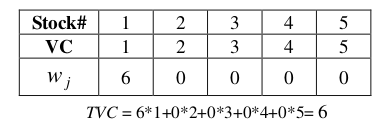
\includegraphics[width=0.45\linewidth]{img/vrednost_resenja_2.png}
    \caption{Računanje vrednosti rešenja}
\end{figure}

\vspace{0.5cm}

\section{Simulirano kaljenje}
Simulirano kaljenje je metaheuristički algoritam za rešavanje optimizacionih problema, inspirisan procesom kaljenja metala u metalurgiji. Cilj algoritma je pronaći globalni optimum funkcije, izbegavajući zaglavljivanje u lokalnim optimumima.

Algoritam započinje od početnog rešenja i iterativno ga poboljšava. U svakoj iteraciji, trenutno rešenje se modifikuje i evaluira se ciljna funkcija. Ako je novo rešenje bolje, ono se prihvata. Međutim, ako je novo rešenje lošije, ono se prihvata sa određenom verovatnoćom, koja opada tokom izvršavanja algoritma. Ova verovatnoća prihvatanja lošijih rešenja omogućava algoritmu da izađe iz lokalnih optimuma i istraži širi prostor rešenja. \\

\subsection{Parametri i funkcije}
U ovom radu, za implementaciju simuliranog kaljenja korišćeni su sledeći parametri:
\begin{enumerate}
	\item Početna temperatura
	\item Minimalna temperatura
	\item Alfa: koristi se za izračunavanje sledeće vrednosti temperature. Ima vrednost između 0 i 1
	\item Maksimalan broj iteracija
	\item Maksimalan broj prihvaćenih rešenja tokom trenutne temperature \\
\end{enumerate}

Takođe su testirane dve različite funkcije za izračunavanje naredne vrednosti temperature:
\begin{enumerate}
	\item \textit{calc\_temperature\_1}:  $[  T_{next} = \frac{T_{current}}{1 + \alpha \cdot T_{current}} ]$, $[\alpha = \frac{T_0 - T_{min}}{N \cdot T_0 \cdot T_{min}}]$

	\item \textit{calc\_temperature\_2}: $[T_{next} = \alpha \cdot T_{current} ]$, $ \alpha$ je odabrana fiksna vrednost
\end{enumerate}

Testirane su i tri funkcije za kreiranje novog rešenja:
\begin{enumerate}
	\item \textit{Swap}
	\item \textit{Insert}
	\item \textit{Inverse} 
\end{enumerate}


\vspace{0.5cm}
\begin{center}
  \hspace{1cm}
  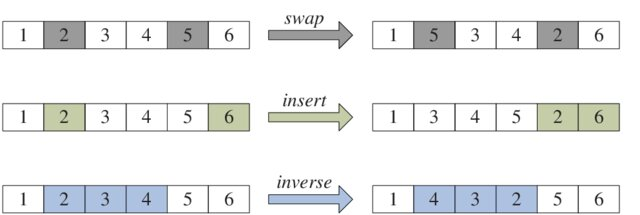
\includegraphics[width=0.8\linewidth]{img/make_sc_funs.jpg}
  \hspace{1cm} 
\end{center}
\vspace{0.5cm}

\subsection{Testiranje i odabir parametara i funkcija}
Za biranje početne temperature, minimalne temperature, i maksimalan broj prihvaćenih rešenja po temperaturi pokrenut je \textit{grid search} nad svim test primerima. Izabrana početna temperatura je 100, minimalna temperatura 1, a maksimalan broj prihvaćenih rešenja po temperaturi 2.

Zatim su testirane dve funkcije za smanjivanje temperature. Za prvu varijantu se alfa računa po formuli, a za drugu varijantu su testirane sledeće vrednosti: 0.95, 0.98, 0.99, 0.999. Za svaku kombinaciju odabrane funkcije i vrednosti alfa je algoritam pokrenut po 5 puta nad svim test primerima. Bolje rezultate je ostvarila prva funkcija.

Na isti način su testirane i funkcije za kreiranje novog rešenja: za svaku funkciju su po 5 puta pokrenuti svi test primeri. Funkcija \textit{swap} je imala najbolje rezultate.

Radi odabira broja iteracija je algoritam pušten nad svim test primerima, i izračunata je prosečna vrednost rešenja po iteracijama, kao i prosečno procentualno poboljšanje rešenja po iteracijama u odnosu na početno rešenje.

\vspace{0.5cm}
\begin{center}
  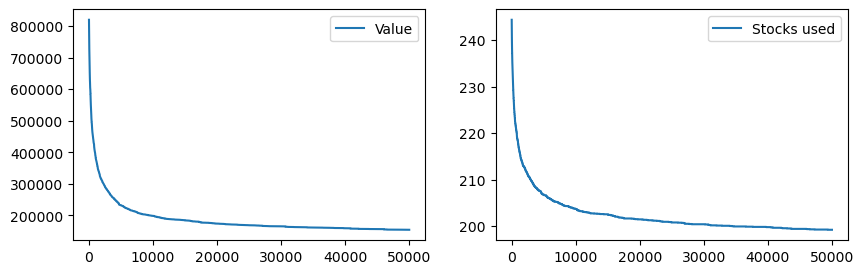
\includegraphics[width=\linewidth]{img/sa_iters_avg.png}
  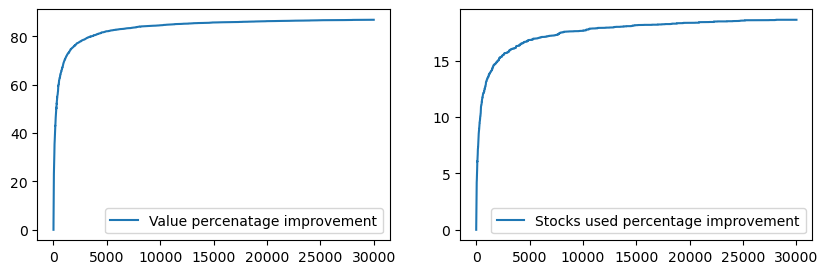
\includegraphics[width=\linewidth]{img/sa_iters_perc.png}
\end{center}
\vspace{0.5cm}

\section{Genetski algoritam}
Genetski algoritam je optimizaciona tehnika inspirisana principima prirodne selekcije i genetike. Pripada široj klasi evolutivnih algoritama, koji koriste mehanizme poput mutacije, ukrštanja i selekcije kako bi iterativno poboljšali rešenja problema.

Osnovni koncept genetskih algoritama je da se potencijalna rešenja problema kodiraju kao hromozomi ili genomi, a zatim se iterativno primenjuju genetski operatori kako bi se stvorile nove generacije rešenja. Svaka generacija se evaluira na osnovu funkcije prilagođenosti (\textit{fitness} funkcije), koja meri kvalitet svakog rešenja u odnosu na definisani problem.

Proces započinje inicijalizacijom početne populacije slučajno generisanih rešenja. Zatim se kroz više iteracija primenjuju funkcije selekcije, ukštanja i mutacije, postepeno evoluirajući populaciju ka boljim rešenjima.

\subsection{Parametri i funkcije}
Za implementaciju genetskog algoritma korišćeni su sledeći parametri:
\begin{enumerate}
	\item Veličina populacije
	\item Elitizam
	\item Mutacija i ukrštanje
		\begin{itemize}
			\item DHM/ILC (Decreasing High Mutation Rate (DHM) and an Increasing Low Crossover Rate (ILC))
			\item ILM/DHC (Increasing Low Mutation Rate (ILM) and a Decreasing High Crossover Rate (DHC))
			\item Fiksna verovatnoća mutacije i ukrštanja
		\end{itemize}
	\item Broj iteracija
	\item Veličina turnira (turnirska selekcija)
	\item Selekcioni pritisak (rangovska selekcija) \\
\end{enumerate}

Testirane su tri funkcije selekcije:
\begin{enumerate}
	\item Turnirska selekcija
	\item Ruletska selekcija
	\item Rangovska selekcija \\
\end{enumerate}

Testirane su tri funkcije ukrštanja, ali zbog toga što nisu direktno primenjive na originalno rešenje, bilo je potrebno prvo modifikovati ih.

\vspace{0.5cm}
\begin{center}
  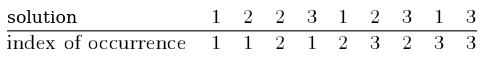
\includegraphics[width=0.8\linewidth]{img/modifikacija_resenja.png}
\end{center}
\vspace{0.5cm}


Tri funkcije ukrštanja:
\begin{enumerate}
	\item \textit{Partially mapped crossover}

	\vspace{0.5cm}
	\begin{center}
	  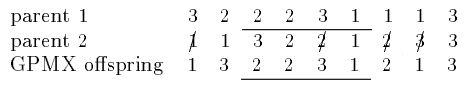
\includegraphics[width=0.8\linewidth]{img/partially_mapped_crossover.png}
	\end{center}
	\vspace{0.5cm}

	\item \textit{Generalized order crossover}

	\vspace{0.5cm}
	\begin{center}
	  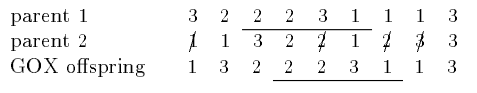
\includegraphics[width=0.8\linewidth]{img/generalized_order_crossover.png}
	\end{center}
	\vspace{0.5cm}

	\item \textit{Precedence preservative crossover}

	\vspace{0.5cm}
	\begin{center}
	  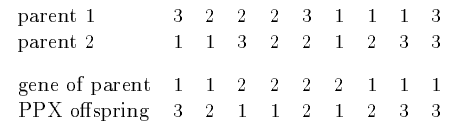
\includegraphics[width=0.8\linewidth]{img/precedence_preservative_crossover.png}
	\end{center}
	\vspace{0.5cm}

\end{enumerate}



 Četiri funkcije mutacije:
\begin{enumerate}
	\item \textit{Swap}
	\item \textit{Insert}
	\item \textit{Inverse} 
	\item \textit{Shuffle} \\
\end{enumerate}

\subsection{Testiranje i odabir parametara i funkcija}
Zbog dugačkog vremena izvršavanja, odabrana je fiksna veličina populacije od 100 jedinki. 

Prvo je pokrenut \textit{random search} nad svim test primerima, sa 150 kombinacija parametara koji se tiču elitizma, ukrštanja, i mutacije. Pristup sa fiksnom verovatnoćom mutacije i ukrštanja se pokazao bolje od druga dva pristupa, dok za elitizam nije mogao da se izvede definitivan zaključak.

Za verovatnoću mutacije su testirane vrednosti od 0.03 do 0.08. Za svaku verovatnoću su pokrenuti svi test primeri po 3 puta. Najbolji rezultati su ostvareni sa verovatnoćom 0.07.

Za verovatnoću ukrštanja su testirane vrednosti od 0.6 do 1, i za svaku verovatnoću su takođe pokrenuti svi test primeri po 3 puta. Vrednost 0.85 je ostvarila najbolje rezultate.

Radi biranja najboljih funkcija selekcije, ukrštanja i mutacije pokrenut je \textit{grid search}, gde je ispitana svaka kombinacija ovih funkcija nad svim test primerima. Sa rezultatima su se istakle kombinacije sa turnirskom selekcijom i \textit{swap} funkcijom mutacije, dok za funkciju ukrštanja nije moglo da se dođe do definitivnog zaključka: \textit{precedence preservative crossover} je imao najbrže vreme izvršavanja, ali najgore rezultate, dok između ostale dve funkcije nije mogla da se primeti značajna razlika u rezultatima. Zato je za obe funkcije algoritam pokrenut nad svim test primerima po 3 puta. Ovog puta je \textit{generalized order crossover} ostvario najbolje rezultate. 

Za elitizam su testirane veličine od 0 do 10\% od ukupnog broja populacije, gde je veličina od 4\% ostvarila najbolje rezultate. Takođe su testirane različite veličine turnira za selekciju. Odabrana je veličina od 6 jedinki po turniru.

Radi odabira broja iteracija genetski algoritam je pokrenut nad svim test primerima, i izračunata je prosečna vrednost najboljeg rešenja populacije, po svakoj iteraciji. Konačno odabran broj iteracija je 600.

\vspace{0.5cm}
\begin{center}
  \hspace{1cm}
  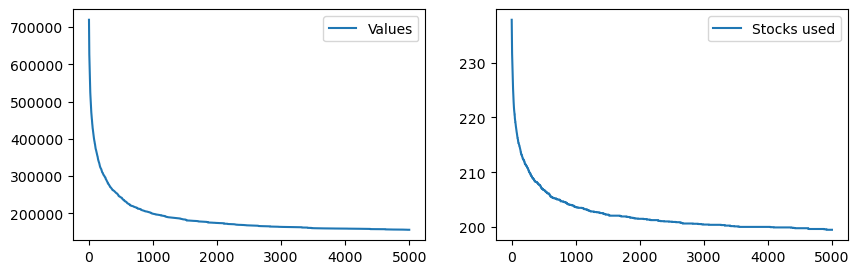
\includegraphics[width=\linewidth]{img/ga_iters.png}
  \hspace{1cm} 
\end{center}
\vspace{0.5cm}

\section{Kombinacija genetskog algoritma i simuliranog kaljenja}

Testirane su tri varijante kombinacije genetskog algoritma i simuliranog kaljenja. U prvoj varijanti se simulirano kaljenje pokreće nad svakom jedinkom populacije u svakoj iteraciji tokom genetskog algoritma. 

\vspace{0.5cm}
\begin{center}
  \hspace{1cm}
  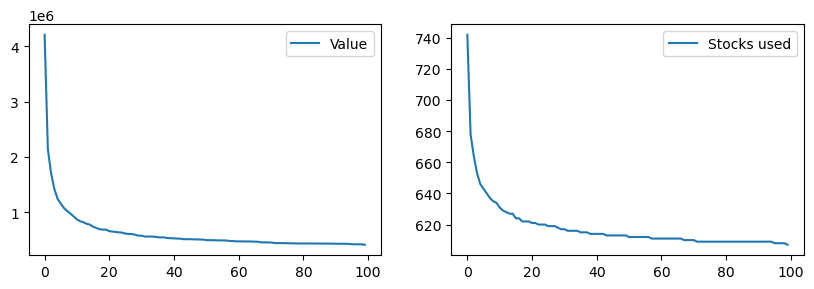
\includegraphics[width=\linewidth]{img/ga_sa_1.png}
  \hspace{1cm} 
\end{center}
\vspace{0.5cm}

U drugoj varijanti se simulirano kaljenje pokreće samo nad najboljom jedinkom populacije u svakoj iteraciji.

\vspace{0.5cm}
\begin{center}
  \hspace{1cm}
  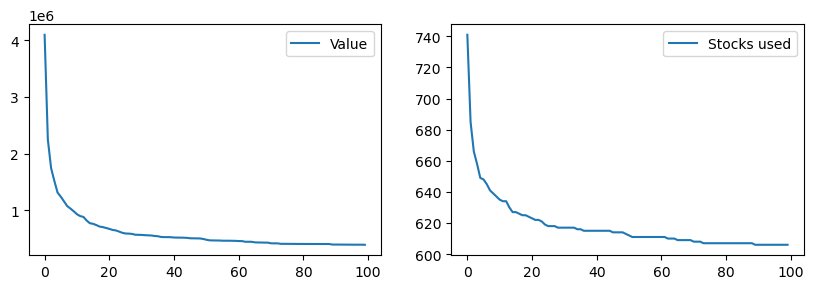
\includegraphics[width=\linewidth]{img/ga_sa_2.png}
  \hspace{1cm} 
\end{center}
\vspace{0.5cm}

U trećoj varijanti je simulirano kaljenje pokrenuto nad konačnim rešenjem genetskog algoritma.

\vspace{0.5cm}
\begin{center}
  \hspace{1cm}
  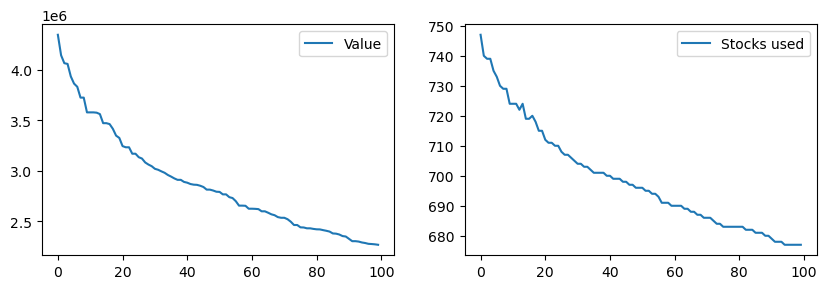
\includegraphics[width=\linewidth]{img/ga_sa_3.png}
  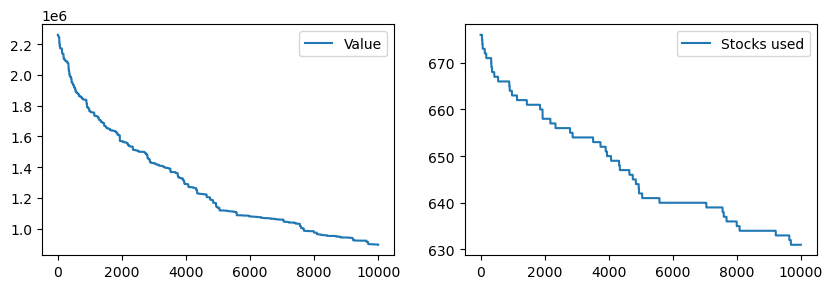
\includegraphics[width=\linewidth]{img/ga_sa_3_part2.png}
  \hspace{1cm} 
\end{center}
\vspace{0.5cm}

Prva i druga varijanta su ostvarile slične rezultate, značajno bolje od treće. Vreme izvršavanja druge varijante je neuporedivo manja od vremena izvršavanja prve varijante.


\section{Poređenje rezultata}

Poređeni su rezultati CPLEX rešavača, simuliranog kaljenja, genetskog algoritma, i druge varijante kombinacije genetskog algoritma i simuliranog kaljenja. Izlaz CPLEX rešavača nije vrednost rešenja kao kod ostalih algoritama, nego broj iskorišćenih komada materijala. Pokrenut je nad prvih 15 test primera, jer je na ostalim previše dugo vreme izvršavanja, a ostali algoritmi su pokrenuti nad svim test primerima.

Na svim test primerima je najbolju vrednost rešenja imala kombinacija algoritama, gde je simulirano kaljenje imalo jednak rezultat na dva test primera, i genetski algoritam na jednom.

\vspace{0.5cm}
\begin{center}
  \hspace{1cm}
  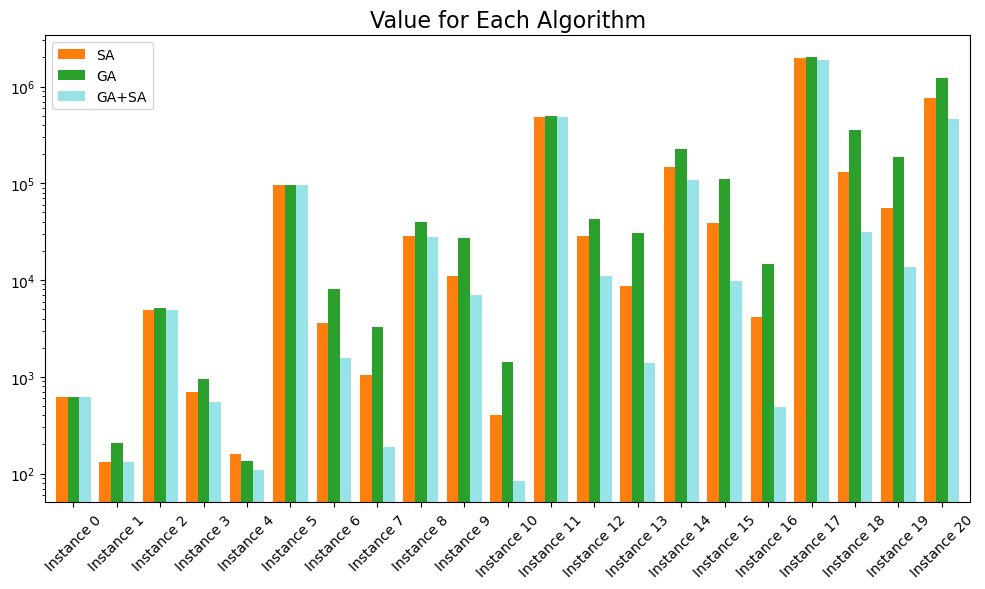
\includegraphics[width=\linewidth]{img/comparison_value.png}
  \hspace{1cm} 
\end{center}
\vspace{0.5cm}

Za broj iskorišćenih komada materijala je takođe kombinacija algoritama imala najbolje rešenje, gde je CPLEX imao jednak rezultat na 2 test primera, simulirano kaljenje na 8, i genetski algoritam na 6.

\vspace{0.5cm}
\begin{center}
  \hspace{1cm}
  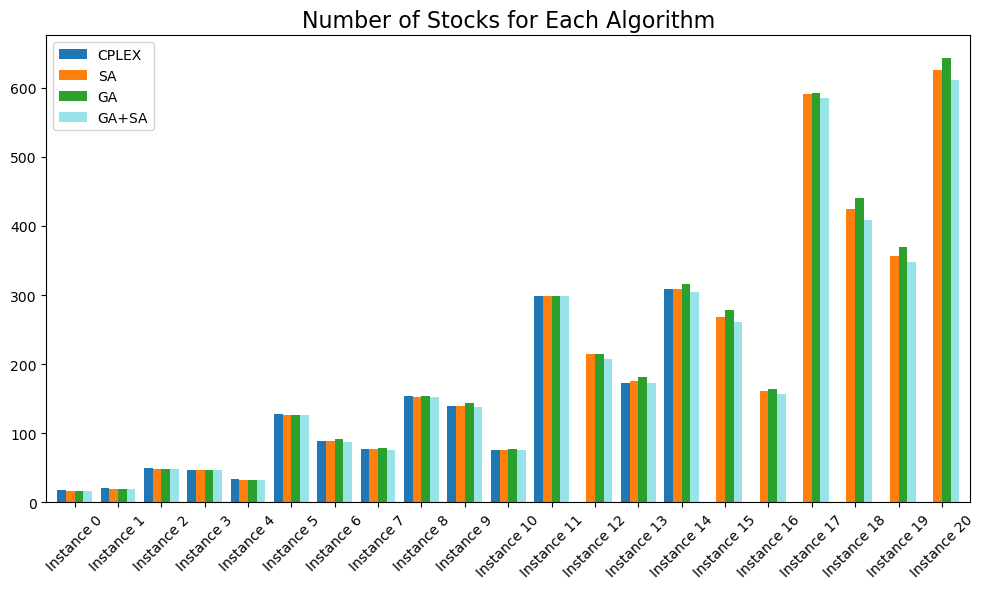
\includegraphics[width=\linewidth]{img/comparison_stocks.png}
  \hspace{1cm} 
\end{center}
\vspace{0.5cm}

Na svim test primerima je najmanje vreme izvršavanja imalo simulirano kaljenje.

\vspace{0.5cm}
\begin{center}
  \hspace{1cm}
  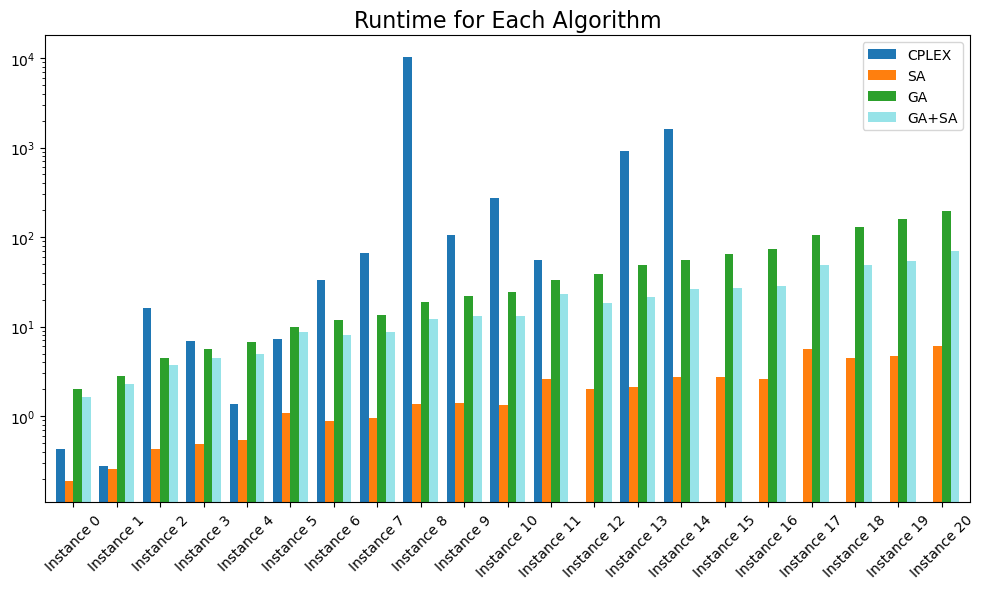
\includegraphics[width=\linewidth]{img/comparison_runtime.png}
  \hspace{1cm} 
\end{center}
\vspace{0.5cm}

\vspace{0.5cm}
\begin{center}
  \hspace{1cm}
  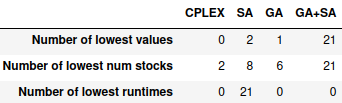
\includegraphics[width=0.6\linewidth]{img/comparison_table.png}
  \hspace{1cm} 
\end{center}
\vspace{0.5cm}

\end{document}